\section{Research Question}
Can feature-guided spatial bias improve boundary accuracy while preserving
overall segmentation quality?

\paragraph{NACLIP baseline.}
In the final visual attention layer, NACLIP adds a fixed Gaussian spatial bias
to the key--key logit $k_i^\top k_j/\sqrt{d}$ before softmax, where $k_i$ and
$k_j$ are the patch keys and $d$ is their dimension per attention head. For
patches at grid positions $p_i$ and $p_j$, the bonus is
\[
    G_{ij} = \exp\!\left(-\frac{\|p_i-p_j\|_2^2}{2\sigma^2}\right).
\]
Nearby patches receive a larger bonus, and equally distant pairs receive the
same bonus even when they lie on opposite sides of a class boundary.

\paragraph{Proposed feature-guided bias.}
We keep the key--key logit and scale the Gaussian bonus using the cosine
similarity $s_{ij}$ between patch features from CLIP's penultimate visual block.
The new spatial bias is
\[
    B_{ij} = G_{ij}\,\mathrm{sigmoid}\!\left(\frac{s_{ij}-\tau}{T}\right),
\]
where $\tau$ is the similarity at which a pair retains half of its Gaussian
bonus and $T$ controls how gradually the gate changes. At the same distance,
dissimilar patches retain less of the bonus, which may reduce information
sharing across class boundaries.

\section{Controlled Setup}
We use the validation splits of ADE20K (ADE in the NACLIP paper) and PASCAL
Context-59 (PC59). Table~\ref{tab:naclip-reported-miou} gives the published
reference scores from Table~1 of Hajimiri et al.\ (WACV 2025), with and without
Pixel-Adaptive Mask Refinement (PAMR). The paper reports mIoU for both settings.

\begin{table}[htbp]
    \centering
    \caption{Validation splits and published NACLIP mIoU (\%).}
    \label{tab:naclip-reported-miou}
    \begin{tabular}{lrrr}
        \hline
        Dataset & Val.\ images & PAMR off & PAMR on \\
        \hline
        ADE20K & 2,000 & 17.4 & 19.1 \\
        PC59   & 5,105 & 35.2 & 38.4 \\
        \hline
    \end{tabular}
\end{table}

We reran the fixed-Gaussian baseline on PC59 to measure boundary and interior
accuracy alongside mean intersection over union (mIoU). The earlier baseline
used PAMR and recorded neither regional accuracy metric. We disabled PAMR in
both the baseline rerun and the feature-guided run to isolate the effect of
changing the spatial bias. The matched PC59 runs used the same validation
images, frozen CLIP ViT-B/16 checkpoint, key--key attention, Gaussian standard
deviation of five patches, preprocessing, sliding-window settings, and
evaluation seed. Both ADE20K conditions also completed the full validation
split.

\paragraph{Boundary and interior accuracy.}
Boundary accuracy was the primary metric because the proposed change targets
errors near class transitions. We scored predictions on the original annotation
grid and excluded ground-truth pixels with the ignore label (255). To build the
boundary band, we marked both pixels in each horizontally or vertically
adjacent pair of valid pixels with different ground-truth labels. The band
contains every valid pixel at a Euclidean distance of at most three pixels from
any marked pixel. The interior contains all remaining valid pixels.

For each region $R$ (boundary or interior), let $C_R$ be the number of pixels
whose predicted class matches the ground-truth class and let $N_R$ be the
total number of valid pixels in that region. We summed both counts across the
validation split before computing the percentage
\[
    \mathrm{Accuracy}_{R} = 100 \times \frac{C_R}{N_R}.
\]
We used mIoU to measure overall segmentation quality. Overall pixel
accuracy (aAcc) is the percentage of correctly classified pixels among all
valid pixels, including both the boundary band and the interior.

\section{Experiments}
\subsection{Implementation details}
Before scoring segmentation, we sampled 32 validation images each from
ADE20K and PC59 without loading their annotation masks. We measured cosine
similarity between patch features from CLIP's penultimate visual block and
pooled the samples with equal weight per image and per dataset. We used two
similarity anchors to set a shared gate for both datasets.

The low anchor $s_{\mathrm{lo}}=0.1140$ was the 10th percentile for pairs at
a Euclidean distance of up to five patch units. The high anchor
$s_{\mathrm{hi}}=0.5411$ was the median for immediately adjacent pairs.
We set the gate to retain 10\% of the Gaussian bonus at the low anchor and
90\% at the high anchor. The sigmoid arguments at those targets are
$-\ln 9$ and $\ln 9$, respectively, giving
\[
    \tau = \frac{s_{\mathrm{lo}}+s_{\mathrm{hi}}}{2} \approx 0.3276,
    \qquad
    T = \frac{s_{\mathrm{hi}}-s_{\mathrm{lo}}}{2\ln 9} \approx 0.0972.
\]
We used $\tau=0.33$ and $T=0.10$ in the segmentation experiments.
Figure~\ref{fig:guidance-calibration} shows the resulting gate over the full
cosine-similarity range. For similarities between $-1$ and $0$, the gate
retains at most 3.6\% of the original Gaussian bonus. It retains 50\% at
$s=0.33$ and reaches 90\% at approximately $s=0.55$.

% Load graphicx in the main Overleaf document's preamble.
\begin{figure}[htbp]
    \centering
    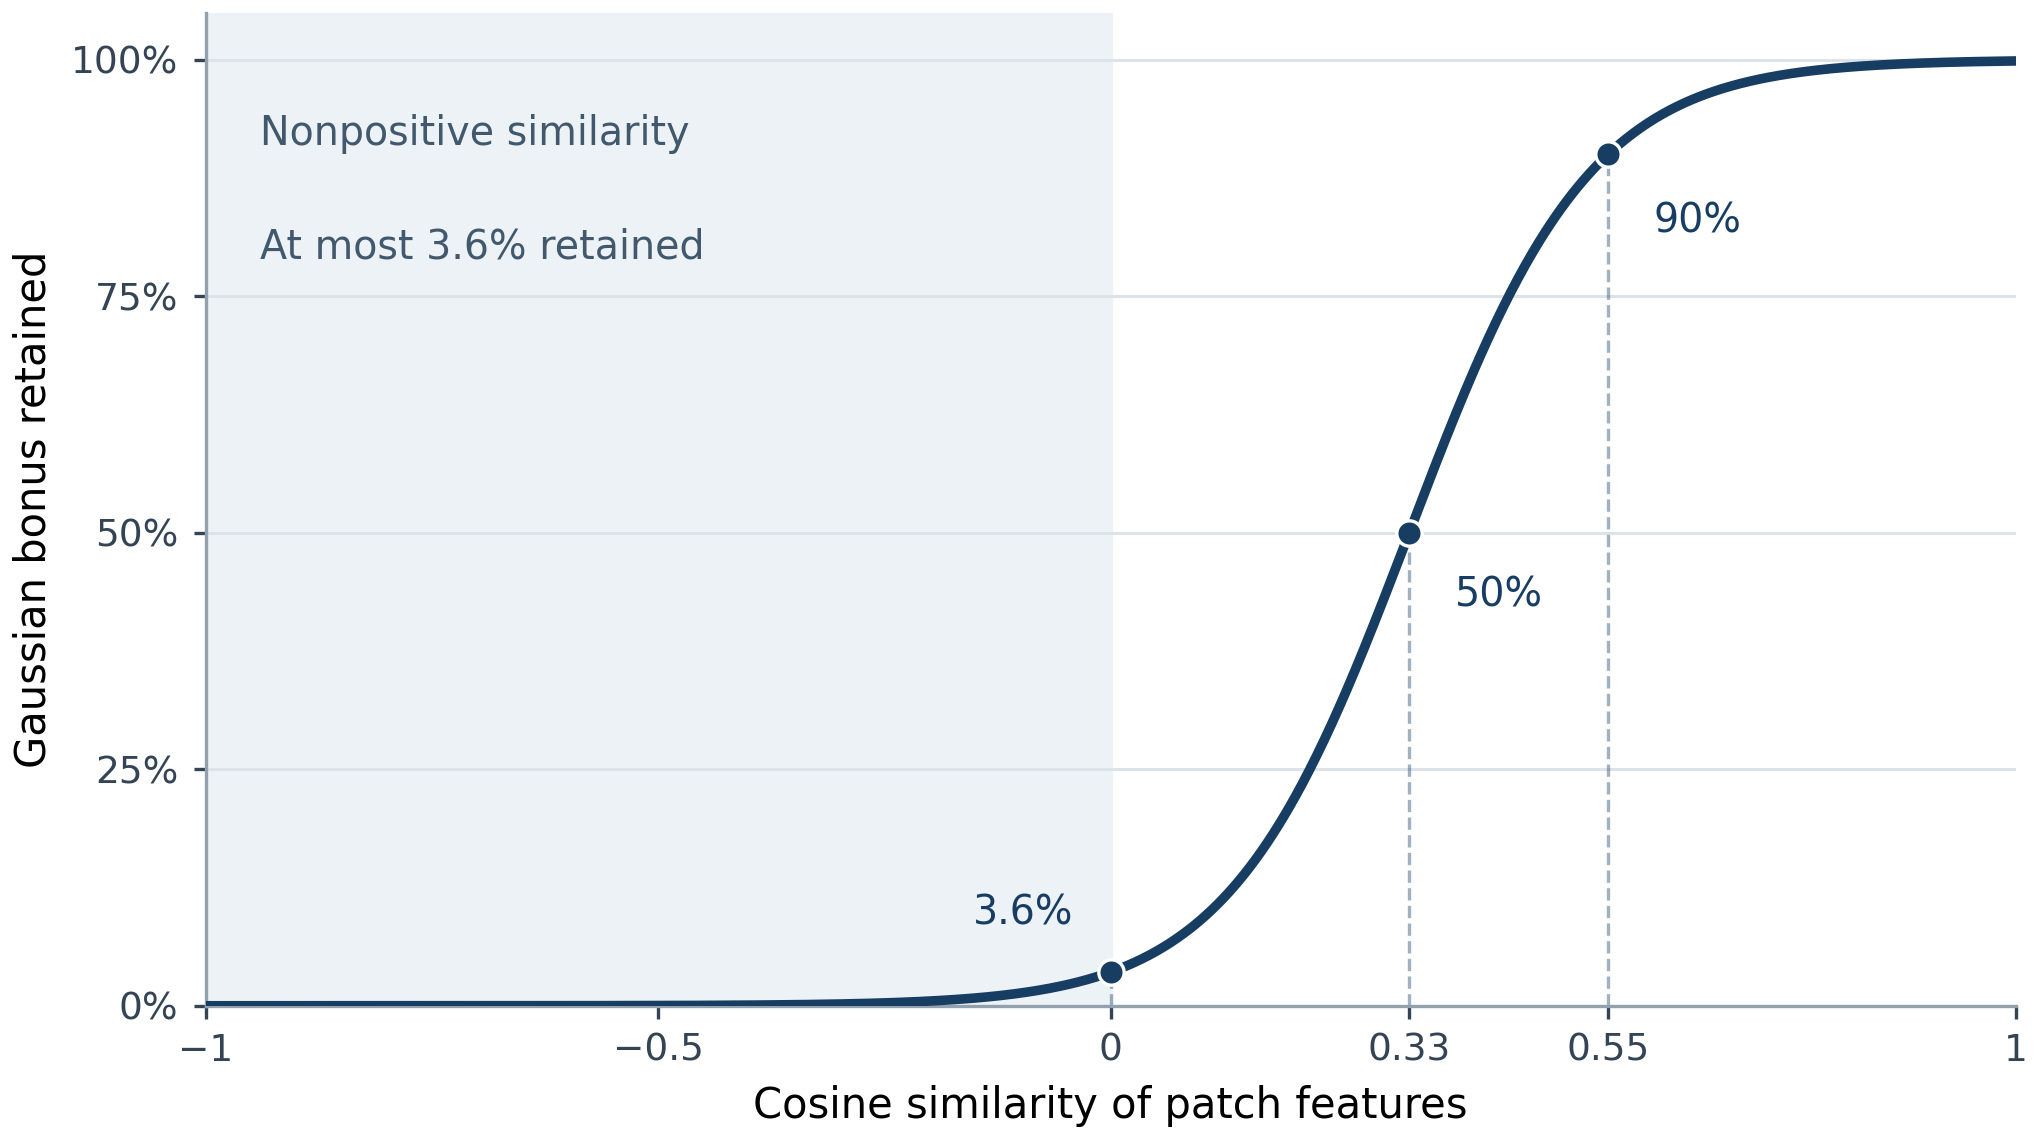
\includegraphics[width=0.8\linewidth]{img/guidance_parameter_selection.jpg}
    \caption{Fraction of the Gaussian spatial bonus retained by the sigmoid
    gate used in the experiments ($\tau=0.33$, $T=0.10$). The shaded region
    highlights nonpositive cosine similarities.}
    \label{fig:guidance-calibration}
\end{figure}

For each patch pair $(i,j)$ in each head of the final visual attention layer,
the fixed and feature-guided logits before the softmax over keys $j$ are
\[
    \begin{array}{rl}
    \ell^{\mathrm{fixed}}_{ij}
      &= \displaystyle\frac{k_i^\top k_j}{\sqrt{d}} + G_{ij}, \\[6pt]
    \ell^{\mathrm{guided}}_{ij}
      &= \displaystyle\frac{k_i^\top k_j}{\sqrt{d}}
        + G_{ij}\,\mathrm{sigmoid}\!\left(\frac{s_{ij}-0.33}{0.10}\right).
    \end{array}
\]

\subsection{Main results}
On PC59, both conditions completed all 5,105 validation images with PAMR
disabled. Feature guidance reduced boundary accuracy by 0.1248 percentage
points, from 36.3862\% to 36.2615\%. Table~\ref{tab:pc59-results} shows that
mIoU, interior accuracy, and overall pixel accuracy also fell slightly.

\begin{table}[htbp]
    \centering
    \caption{Matched PC59 validation results with PAMR disabled. Changes are
    feature-guided minus fixed Gaussian, in percentage points.}
    \label{tab:pc59-results}
    \begin{tabular}{lrrr}
        \hline
        Metric & Fixed Gaussian & Feature-guided & Change \\
        \hline
        Boundary accuracy (\%) & 36.3862 & 36.2615 & $-0.1248$ \\
        mIoU (\%)              & 35.19   & 34.86   & $-0.33$   \\
        Interior accuracy (\%) & 61.7399 & 61.4408 & $-0.2990$ \\
        aAcc (\%)              & 59.34   & 59.06   & $-0.28$   \\
        \hline
    \end{tabular}
\end{table}

On ADE20K, both runs completed all 2,000 validation images and scored the
same number of boundary and interior pixels. Feature guidance reduced boundary
accuracy by 0.0564 percentage points. Table~\ref{tab:ade20k-results} also
shows small decreases in mIoU, interior accuracy, and overall pixel accuracy.

\begin{table}[htbp]
    \centering
    \caption{ADE20K validation results. Changes are feature-guided minus
    fixed Gaussian, in percentage points.}
    \label{tab:ade20k-results}
    \begin{tabular}{lrrr}
        \hline
        Metric & Fixed Gaussian & Feature-guided & Change \\
        \hline
        Boundary accuracy (\%) & 25.5062 & 25.4498 & $-0.0564$ \\
        mIoU (\%)              & 17.42   & 17.23   & $-0.19$   \\
        Interior accuracy (\%) & 47.4225 & 47.1734 & $-0.2491$ \\
        aAcc (\%)              & 45.17   & 44.94   & $-0.23$   \\
        \hline
    \end{tabular}
\end{table}

\subsection{Qualitative results and attention analysis}
Figure~\ref{fig:segmentation-cases} shows three PC59 images selected to
illustrate different outcomes from a local CPU comparison with PAMR disabled.
The per-image accuracies use the same original-resolution metric definitions
as the full-validation comparison.

\begin{figure}[htbp]
    \centering
    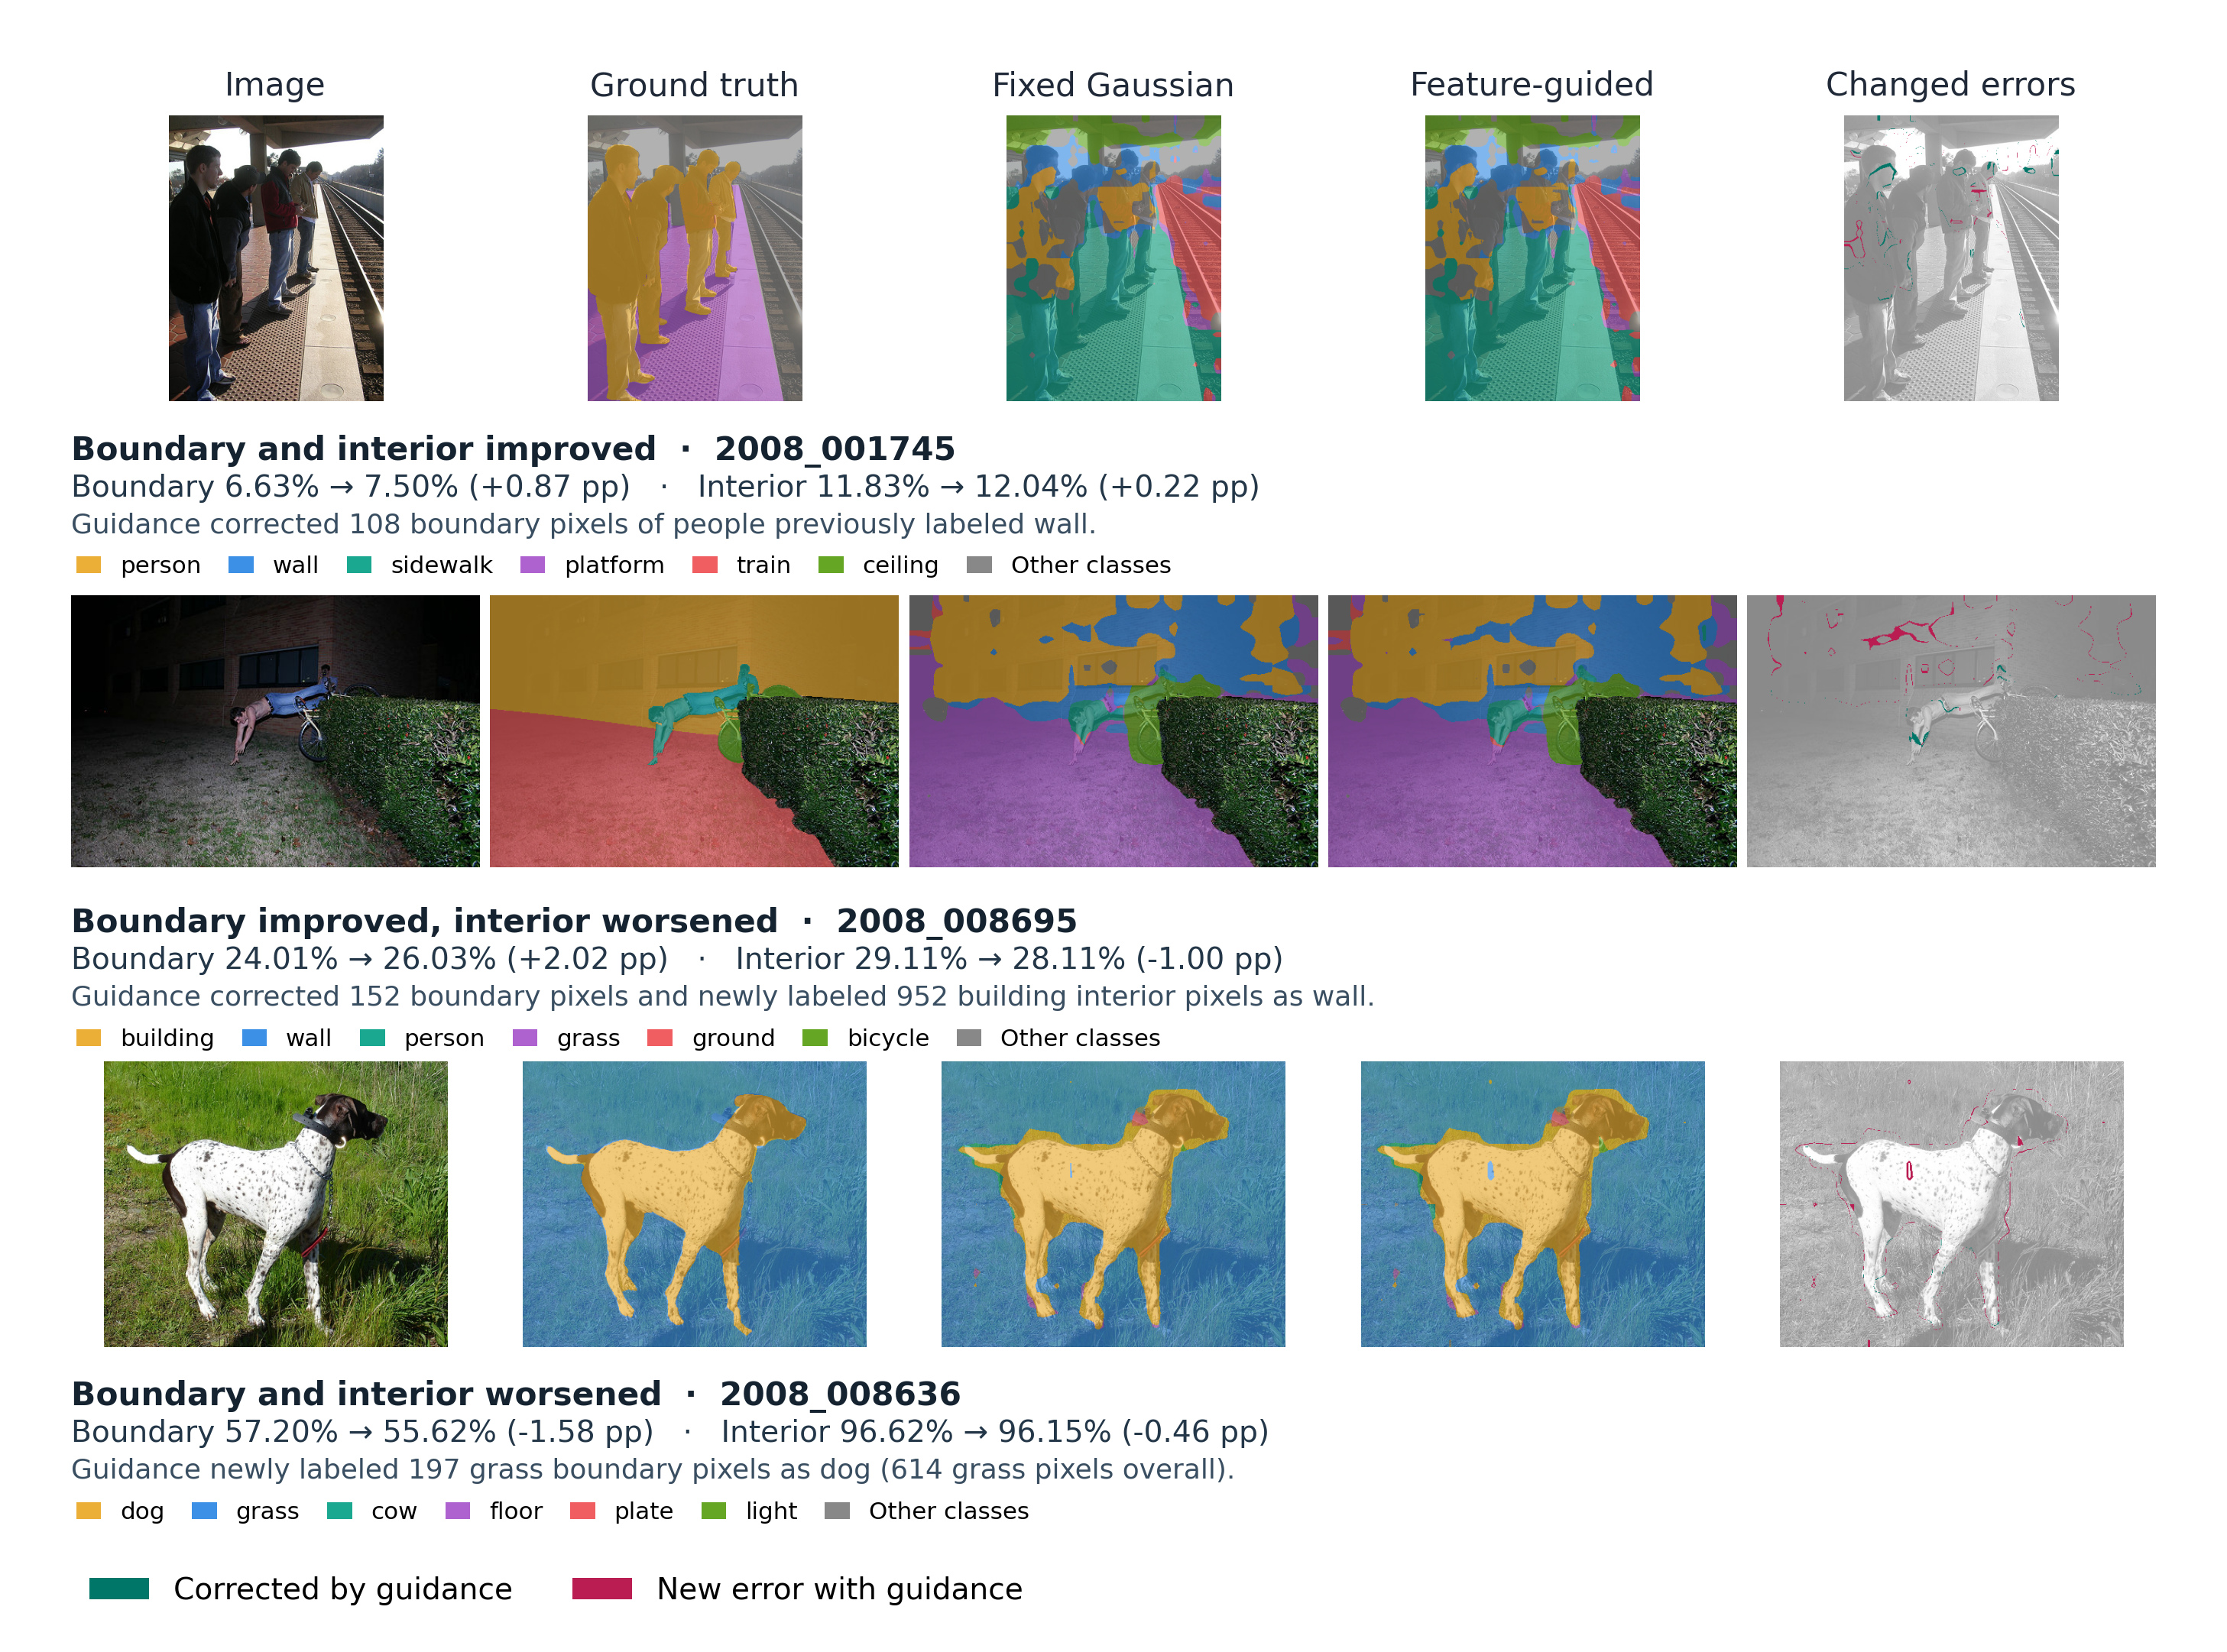
\includegraphics[width=0.8\linewidth]{img/segmentation_case_studies.jpg}
    \caption{Selected PC59 cases from the paired CPU comparison. The
    rightmost column shows pixels whose correctness changed with guidance.
    The examples illustrate distinct outcomes on individual images.}
    \label{fig:segmentation-cases}
\end{figure}

In image \texttt{2008\_001745}, boundary accuracy rose by 0.87 percentage
points and interior accuracy rose by 0.22 points. Guidance correctly labeled
108 boundary pixels of people previously assigned to wall, although overall
accuracy remained low. In \texttt{2008\_008695}, boundary accuracy rose by
2.02 points while interior accuracy fell by 1.00 point. Guidance newly labeled
952 building interior pixels as wall. In \texttt{2008\_008636}, boundary and
interior accuracy fell by 1.58 and 0.46 points, respectively. Guidance newly
labeled 197 grass boundary pixels as dog.

We inspected the final visual layer for one marked query in each of the
person and dog cases. The maps average post-softmax attention across 12
heads. The fixed and guided maps share one probability scale across both
figures, and their overall patterns look similar. The difference panels use
a narrower, shared scale for changes to other patches. The outlined query
is masked in those panels, and its change in self-attention is listed
separately. The class token participates in softmax. The maps display only
patch locations.

\begin{figure}[htbp]
    \centering
    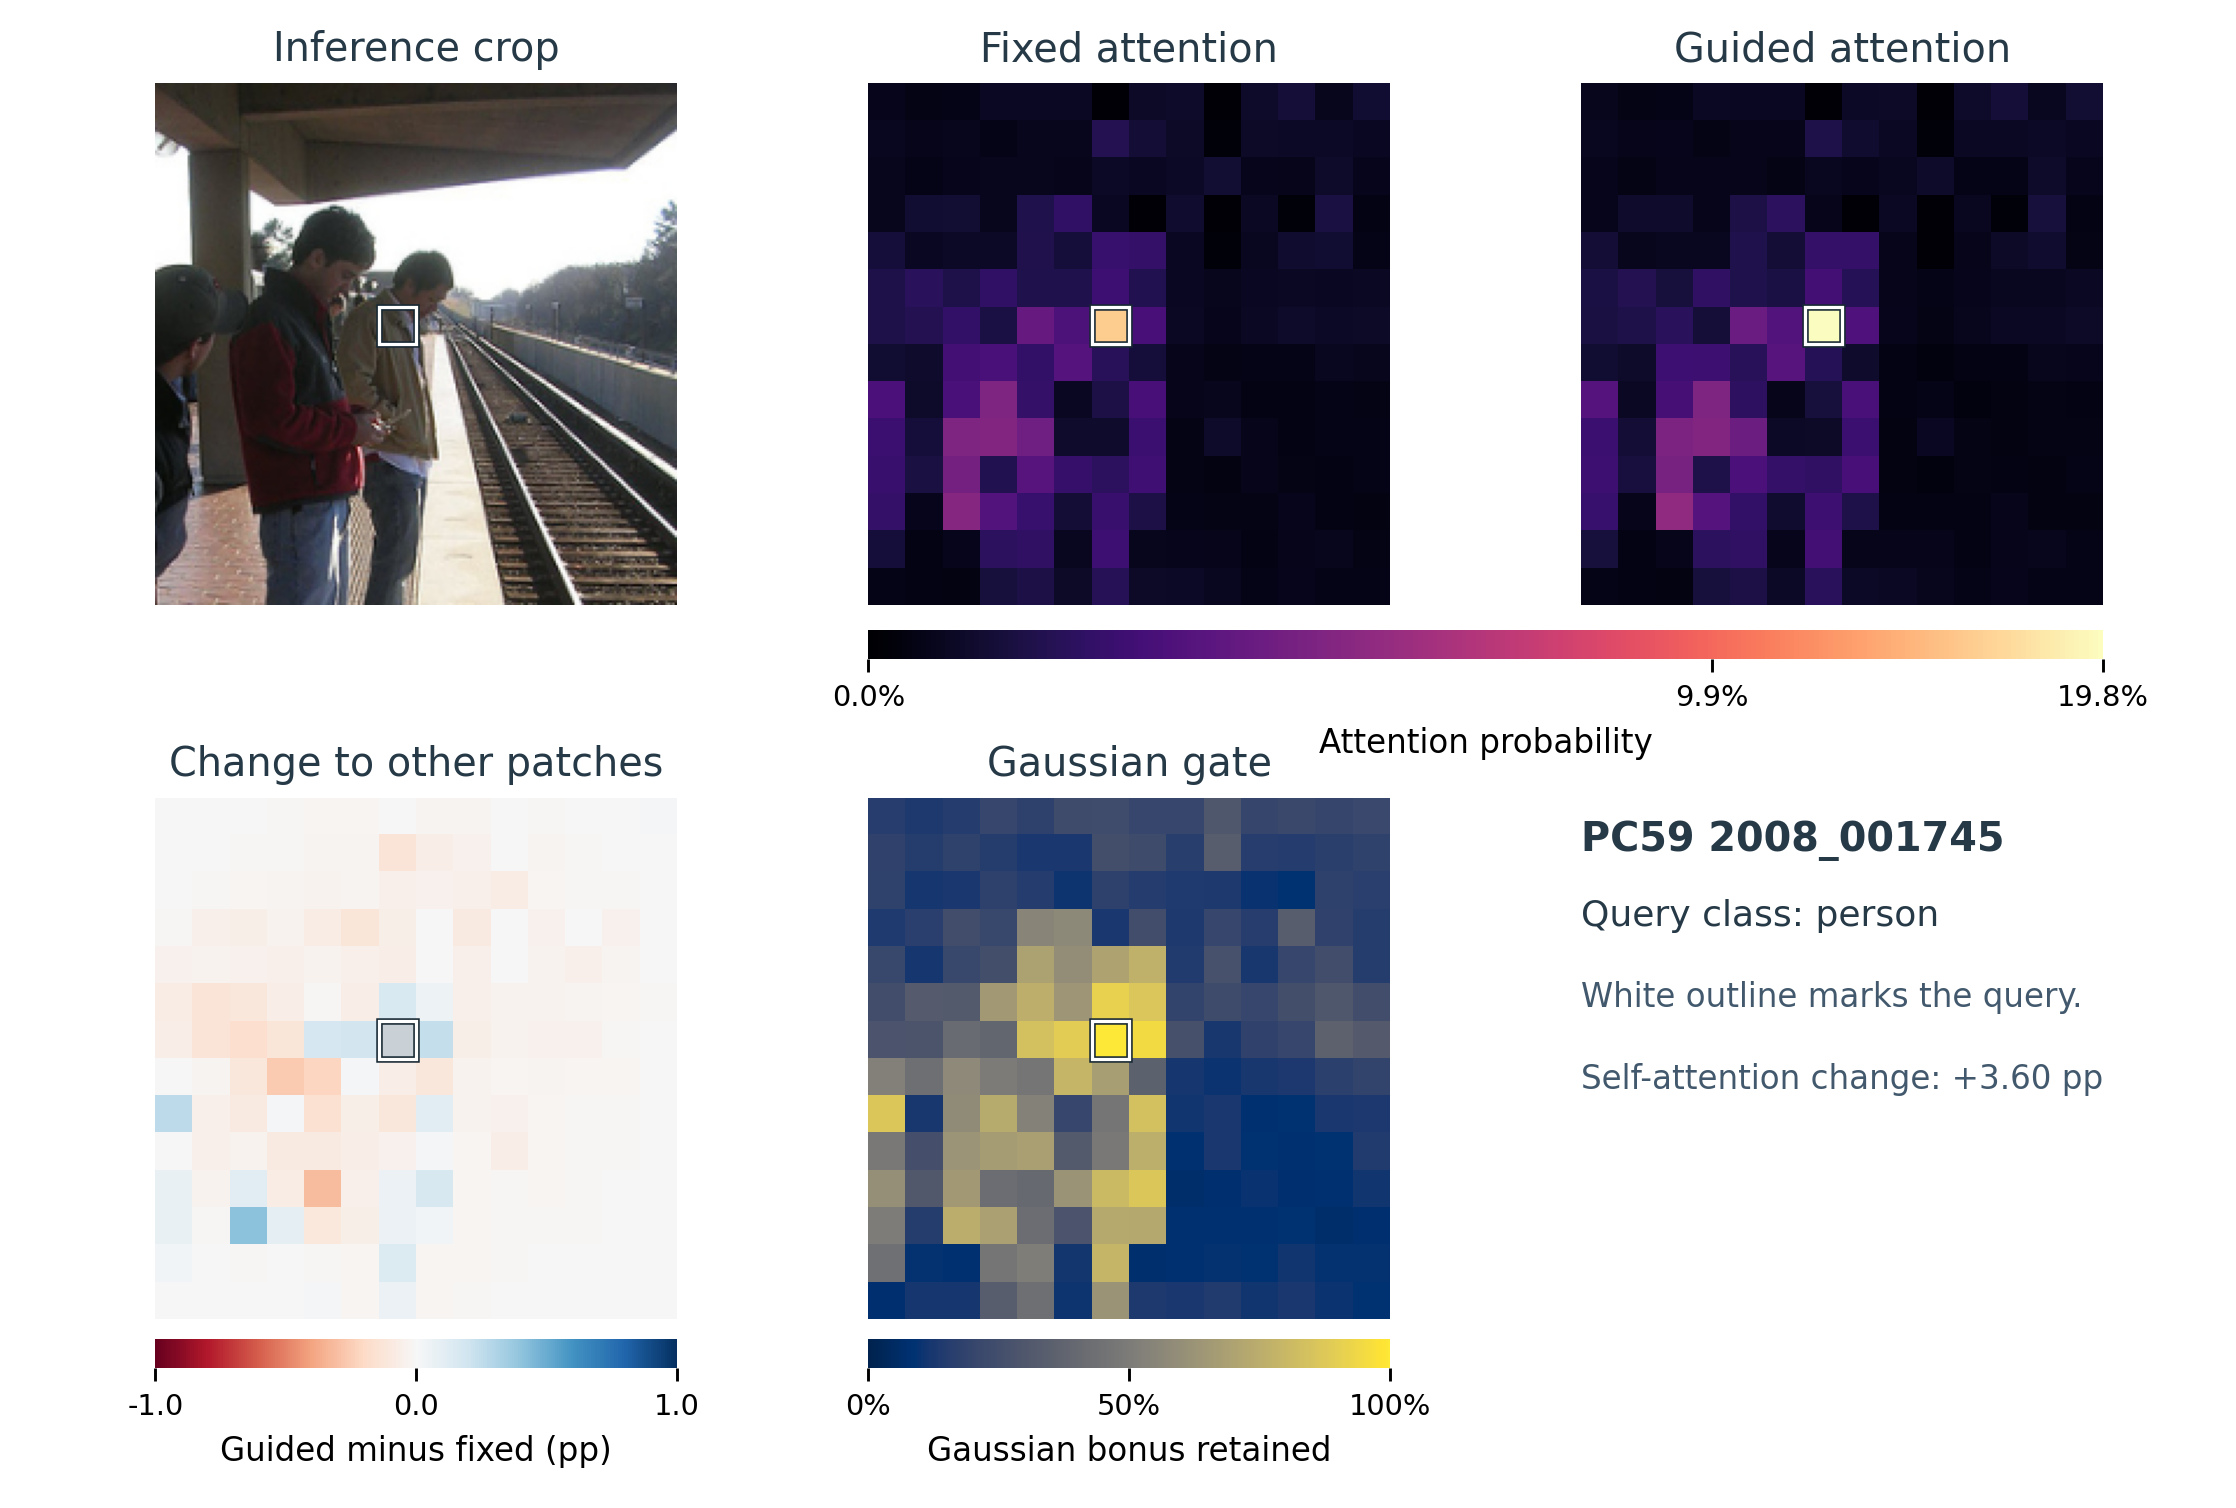
\includegraphics[width=0.8\linewidth]{img/query_attention_person.jpg}
    \caption{Final-layer attention for the marked person patch in the PC59
    image that improved. The gate shows the fraction of the Gaussian bonus
    retained at each patch.}
    \label{fig:query-attention-person}
\end{figure}

We assigned patch classes when at least 85\% of pixels had the same valid
class. For the person query in Figure~\ref{fig:query-attention-person},
total attention to other confidently labeled person patches decreased from
40.0\% to 38.0\%. Attention to confidently labeled patches of other classes
decreased from 12.2\% to 10.5\%.

\begin{figure}[htbp]
    \centering
    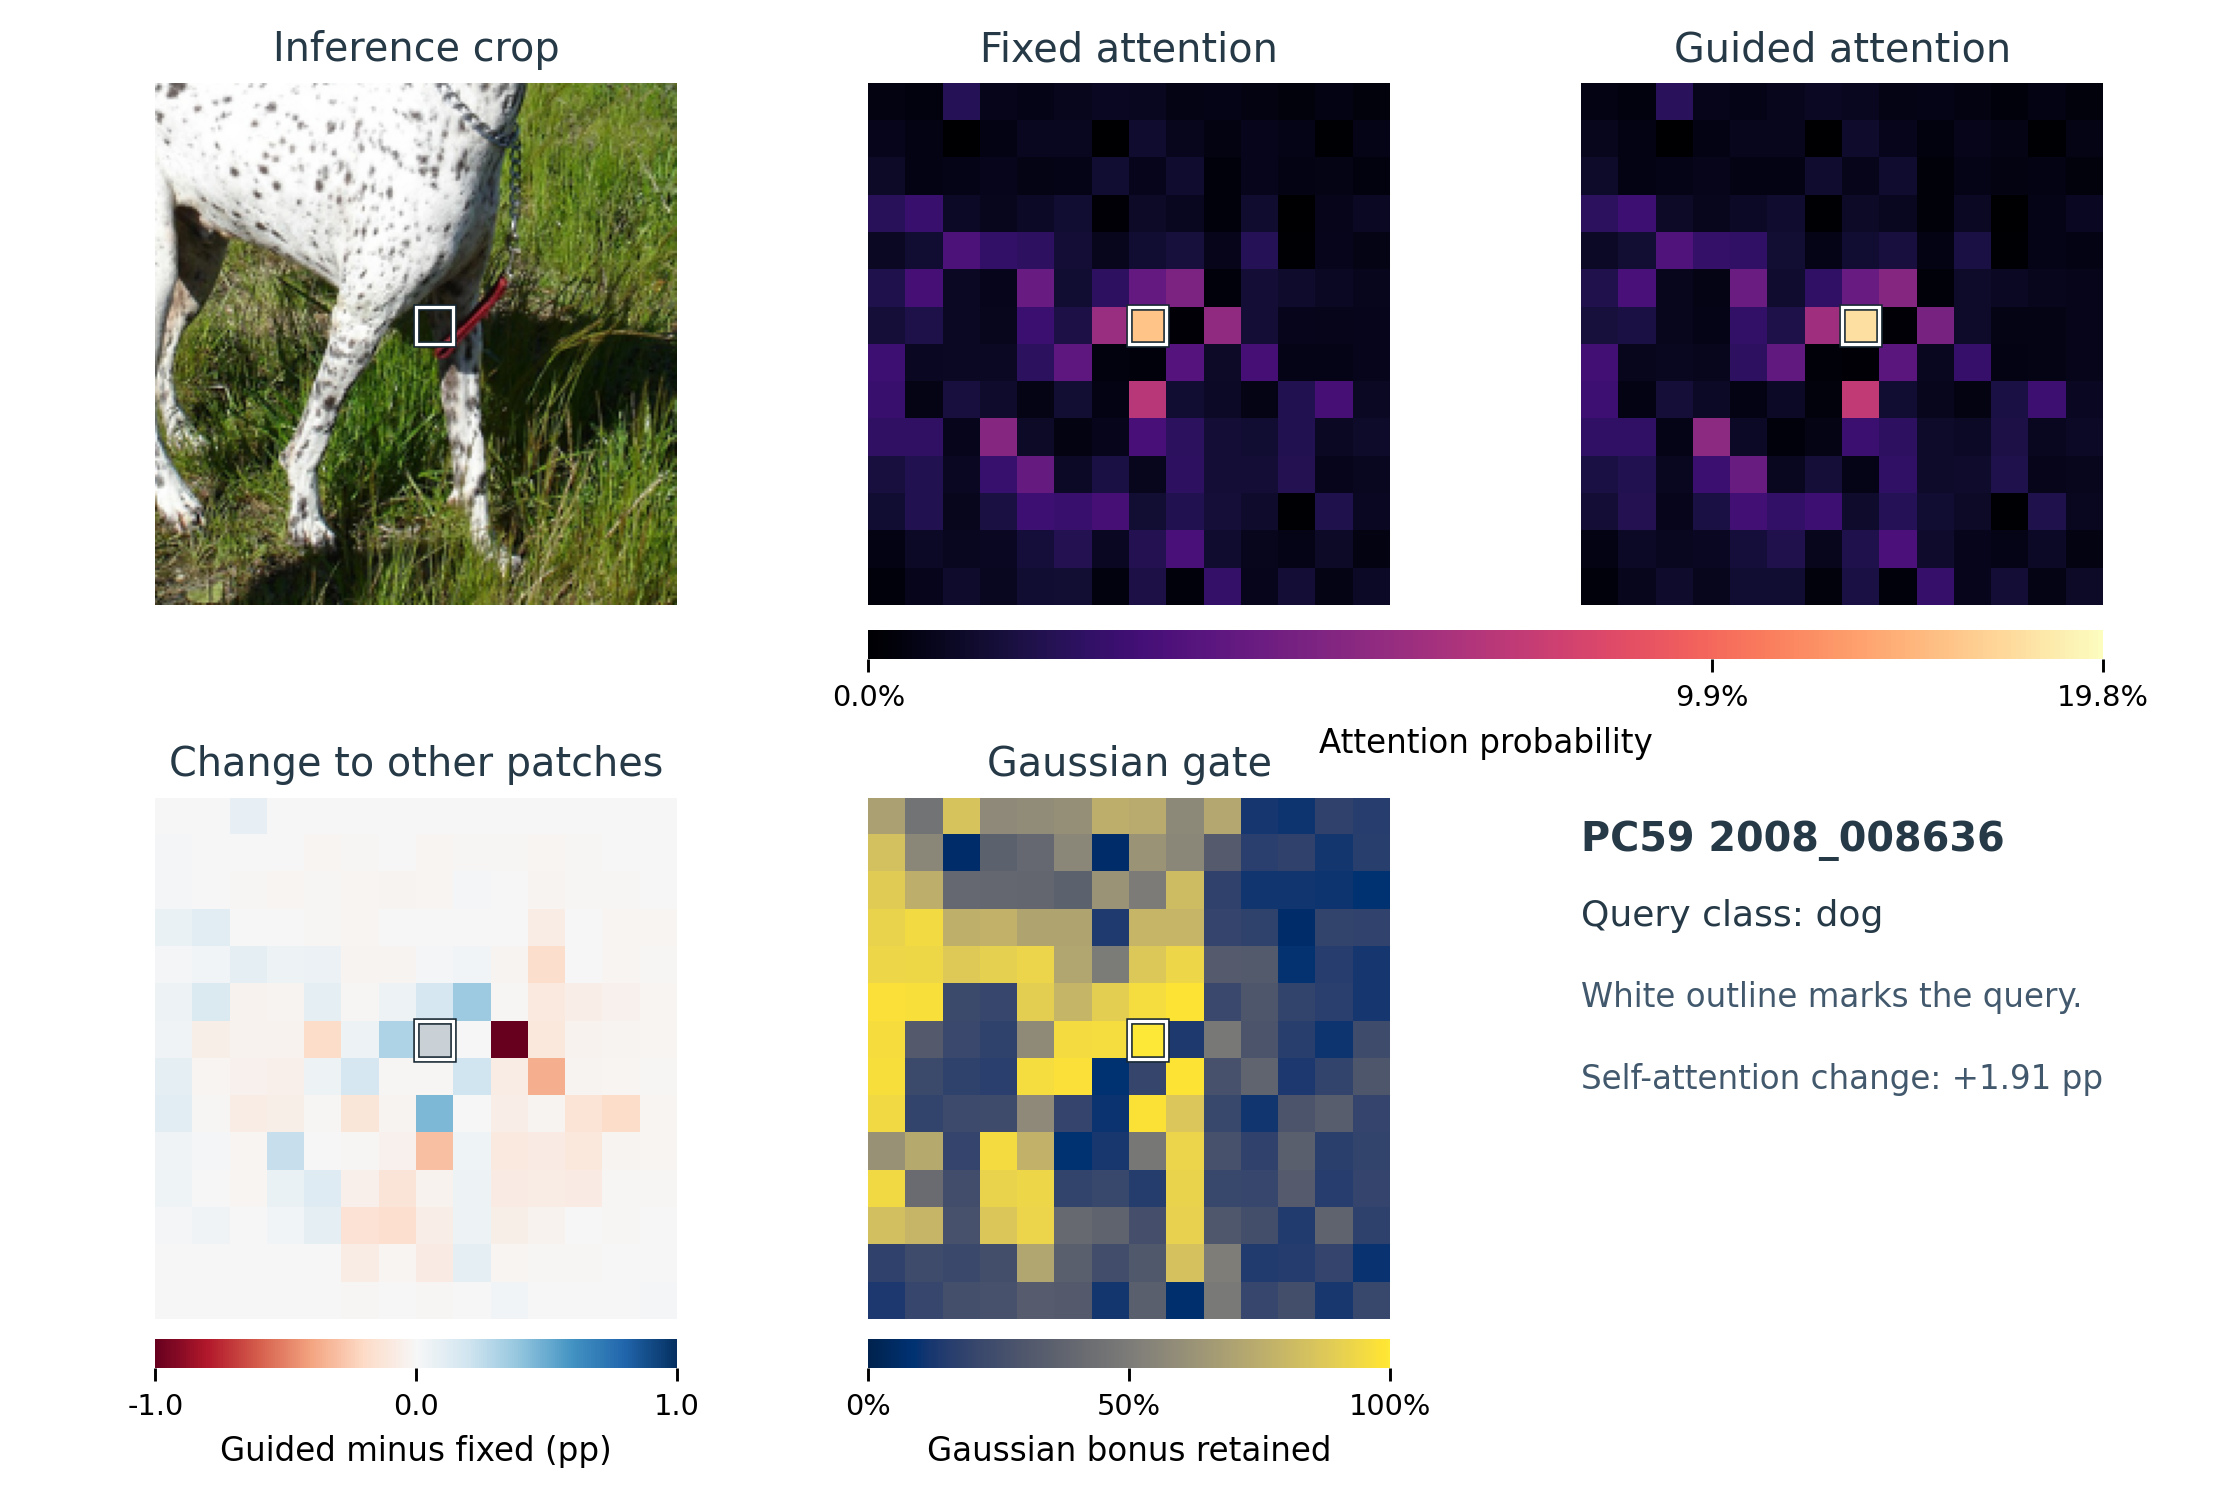
\includegraphics[width=0.8\linewidth]{img/query_attention_dog.jpg}
    \caption{Final-layer attention for the marked dog patch in the PC59
    image that regressed. The signed change shows where other patches gained
    or lost attention probability.}
    \label{fig:query-attention-dog}
\end{figure}

For the dog query in Figure~\ref{fig:query-attention-dog}, attention to
confidently labeled patches of other classes fell from 29.0\% to 24.0\%.
The full-image segmentation still worsened. Each map shows one query in one
crop, and the final mask combines predictions from all patches and
overlapping windows.

To test whether the gate favored same-class pairs, we analyzed one
boundary-rich inference crop from each of 24 exploratory PC59 images.
We compared patch pairs with at least 85\% label agreement within each patch
and averaged across images containing both pair types at the given distance.
For horizontal or vertical neighbors, the mean gate was 0.763 for same-class
pairs and 0.429 for cross-class pairs (22 images). For diagonal neighbors,
the corresponding means were 0.700 and 0.355 (23 images). In these crops,
the gate preferentially retained the bonus for same-class pairs while also
attenuating their spatial support.

\section{Discussion and next steps}
Boundary and interior accuracy both fell slightly on PC59 and ADE20K.
The crop analysis suggests that the gate can distinguish some semantic
transitions, but it also weakens spatial support between patches of the same
class. That weakening could contribute to the observed errors.

In the two attention examples, the fixed and guided maps have similar
spatial patterns. Guidance increased attention to the query itself by
3.60 percentage points in the person crop and 1.91 points in the dog
crop. The change at each other patch was below one point in absolute
value. These examples suggest that the gate can modestly redistribute
attention within an existing pattern. A larger sample is needed to assess
how common this behavior is and how it relates to segmentation accuracy.

The next experiment should compare four conditions on a held-out,
preselected image subset with PAMR disabled. Use the fixed Gaussian, no
spatial bias, the current feature-guided gate, and a constant attenuation
matched to the average guided spatial bonus. This would test whether the
similarity signal helps beyond the effect of reducing the Gaussian bonus.
Measure same-class and cross-class gate values at the same patch distance,
record paired per-image boundary and interior accuracy, and report mIoU.

If the gate shows useful selectivity, test a blend that preserves more of
the original spatial support. With $g_{ij}$ denoting the current sigmoid
multiplier, use
\[
    B_{ij}^{\mathrm{blend}} = G_{ij}\bigl[(1-\alpha)+\alpha g_{ij}\bigr],
    \qquad 0\leq\alpha\leq1.
\]
Choose the settings on a separate calibration pool before scoring the
benchmark. Check whether boundary accuracy improves while interior accuracy
and mIoU hold up before expanding the evaluation.
